\documentclass[12pt,a4paper]{article}

\usepackage{amsmath}
\usepackage{graphicx}
\usepackage{float}
\usepackage{geometry}
\usepackage{booktabs}
\usepackage{listings}
\usepackage{xcolor}
\usepackage{amssymb}
\usepackage{float}
\begin{document}
    

\begin{minipage}{0.6\textwidth}

\includegraphics[width=0.5\textwidth]{IIITB-COMET-Logo.png}
\end{minipage}
\begin{minipage}{0.38\textwidth}
\begin{center}
\textbf{DARSI VAMSI}
\newline
\textbf{COMET FWC 071}
\end{center}
\end{minipage}
\section* {EE 2018 Q-14}
Q.In the logic circuit shown in the figure, Y is given by
\begin{center}
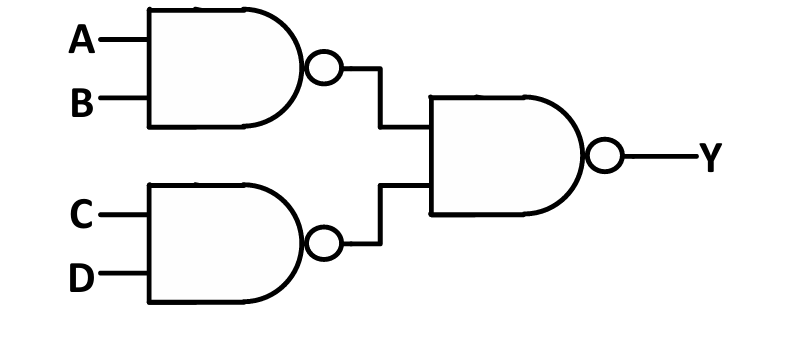
\includegraphics[width=0.75\textwidth]{figure.png}
\begin{enumerate}
\item A) $Y=ABCD$
\item B) $Y=(A+B)(C+D)$
\item C) $Y=A+B+C+D$
\item D) $Y=AB+CD$
\end{enumerate}
\end{center}
\section*{Boolean Expression Derivation}

The given logic circuit consists of three NAND gates.

\subsection*{Step 1: Output of the First Two NAND Gates}

The upper NAND gate produces

\begin{equation}
X = (AB)'
\end{equation}

The lower NAND gate produces

\begin{equation}
W = (CD)'
\end{equation}

\subsection*{Step 2: Output of the Final NAND Gate}

The outputs of the first two NAND gates are connected to a third NAND gate. Therefore,


\section*{Truth Table}

Table~\ref{tab:truth_table} shows the truth table for the Boolean expression
\(Y = AB + CD\).

\begin{table}[H]
\centering
\caption{Truth Table for \(Y = AB + CD\)}
\label{tab:truth_table}
\begin{tabular}{|c|c|c|c|c|c|c|}
\hline
A & B & C & D & AB & CD & Y \\ \hline
0 & 0 & 0 & 0 & 0 & 0 & 0 \\ \hline
0 & 0 & 0 & 1 & 0 & 0 & 0 \\ \hline
0 & 0 & 1 & 0 & 0 & 0 & 0 \\ \hline
0 & 0 & 1 & 1 & 0 & 1 & 1 \\ \hline
0 & 1 & 0 & 0 & 0 & 0 & 0 \\ \hline
0 & 1 & 0 & 1 & 0 & 0 & 0 \\ \hline
0 & 1 & 1 & 0 & 0 & 0 & 0 \\ \hline
0 & 1 & 1 & 1 & 0 & 1 & 1 \\ \hline
1 & 0 & 0 & 0 & 0 & 0 & 0 \\ \hline
1 & 0 & 0 & 1 & 0 & 0 & 0 \\ \hline
1 & 0 & 1 & 0 & 0 & 0 & 0 \\ \hline
1 & 0 & 1 & 1 & 0 & 1 & 1 \\ \hline
1 & 1 & 0 & 0 & 1 & 0 & 1 \\ \hline
1 & 1 & 0 & 1 & 1 & 0 & 1 \\ \hline
1 & 1 & 1 & 0 & 1 & 0 & 1 \\ \hline
1 & 1 & 1 & 1 & 1 & 1 & 1 \\ \hline
\end{tabular}
\end{table}

\section*{Minterm Representation}

From the truth table, the output is equal to 1 for the following minterms:

\begin{equation}
m(3,7,11,12,13,14,15)
\end{equation}

Therefore, the canonical Sum-of-Products (SOP) form is

\begin{equation}
Y(A,B,C,D)=\Sigma m(3,7,11,12,13,14,15)
\end{equation}
\section*{Canonical SOP Expression}

From the truth table, the output is equal to 1 for the minterms

\begin{equation}
m(3,7,11,12,13,14,15)
\end{equation}

Therefore,

\begin{equation}
Y(A,B,C,D)=\Sigma m(3,7,11,12,13,14,15)
\end{equation}

Expanding each minterm,

\begin{align}
m_3 &= A'B'CD \
m_7 &= A'BCD \
m_{11} &= AB'CD \
m_{12} &= ABC'D' \
m_{13} &= ABC'D \
m_{14} &= ABCD' \
m_{15} &= ABCD
\end{align}

Hence, the canonical Sum-of-Products (SOP) expression is

\begin{equation}
Y=
A'B'CD+
A'BCD+
AB'CD+
ABC'D'+
ABC'D+
ABCD'+
ABCD
\end{equation}

This expression is obtained directly from the truth table before any Karnaugh Map simplification.

\section*{Algebraic Simplification}

Starting from the canonical SOP expression,

\begin{equation}
Y=
A'B'CD+
A'BCD+
AB'CD+
ABC'D'+
ABC'D+
ABCD'+
ABCD
\end{equation}

\subsection*{Step 1: Group Terms Having Common Literals}

\begin{equation}
Y=
(A'B'CD+A'BCD+AB'CD)
+
(ABC'D'+ABC'D+ABCD'+ABCD)
\end{equation}

\subsection*{Step 2: Factor (CD) from the First Group}

\begin{equation}
Y=
CD(A'B'+A'B+AB')
+
(ABC'D'+ABC'D+ABCD'+ABCD)
\end{equation}

\subsection*{Step 3: Simplify the First Bracket}

Using

\begin{equation}
A'B'+A'B=A'(B'+B)=A'
\end{equation}

Therefore,

\begin{equation}
A'B'+A'B+AB'=A'+AB'
\end{equation}

Using

\begin{equation}
X+YZ=(X+Y)(X+Z)
\end{equation}

\begin{equation}
A'+AB'=(A'+A)(A'+B')
\end{equation}

\begin{equation}
=1(A'+B')
\end{equation}

\begin{equation}
=A'+B'
\end{equation}

Hence,

\begin{equation}
Y=
CD(A'+B')
+
(ABC'D'+ABC'D+ABCD'+ABCD)
\end{equation}

\subsection*{Step 4: Factor (AB) from the Remaining Terms}

\begin{equation}
Y=
CD(A'+B')
+
AB(C'D'+C'D+CD'+CD)
\end{equation}

\subsection*{Step 5: Simplify the Second Bracket}

\begin{equation}
C'D'+C'D=C'(D'+D)=C'
\end{equation}

Similarly,

\begin{equation}
CD'+CD=C(D'+D)=C
\end{equation}

Therefore,

\begin{equation}
C'D'+C'D+CD'+CD=C'+C
\end{equation}

\begin{equation}
=1
\end{equation}

Hence,

\begin{equation}
Y=CD(A'+B')+AB
\end{equation}

\subsection*{Step 6: Expand the First Term}

\begin{equation}
Y=A'CD+B'CD+AB
\end{equation}

\subsection*{Step 7: Apply Absorption and Consensus Theorem}

Consider

\begin{equation}
Y=AB+A'CD+B'CD
\end{equation}

Using the Consensus Theorem,

\begin{equation}
XY+X'Z+YZ=XY+X'Z
\end{equation}

Let

\begin{equation}
X=A,\qquad Y=B,\qquad Z=CD
\end{equation}

Then,

\begin{equation}
AB+A'CD+BCD=AB+A'CD
\end{equation}

Since

\begin{equation}
B'CD+BCD=CD
\end{equation}

the expression simplifies to

\begin{equation}
AB+CD(A'+B')
\end{equation}

which reduces to

\begin{equation}
\boxed{Y=AB+CD}
\end{equation}

\section*{Karnaugh Map Simplification}

The K-map contains 1's at the minterms

\begin{equation}
m(3,7,11,12,13,14,15)
\end{equation}

\subsection*{Group 1}

Grouping

\begin{equation}
m(12,13,14,15)
\end{equation}

gives

\begin{equation}
AB
\end{equation}

\subsection*{Group 2}

Grouping

\begin{equation}
m(3,7,11,15)
\end{equation}

gives

\begin{equation}
CD
\end{equation}

Combining the groups,

\begin{equation}
\boxed{Y=AB+CD}
\end{equation}
\section*{Hardware Connections}

\subsection*{Arduino Input Generation}

The Arduino Uno is used to generate the four input variables \(A\), \(B\), \(C\), and \(D\) automatically.

\begin{table}[H]
\centering
\caption{Arduino Input Connections}
\label{tab:arduino_inputs}
\begin{tabular}{|c|c|}
\hline
\textbf{Arduino Pin} & \textbf{Logic Variable} \\ \hline
D9  & A \\ \hline
D10 & B \\ \hline
D11 & C \\ \hline
D12 & D \\ \hline
\end{tabular}
\end{table}

\subsection*{Arduino to SN74LS47N Connections}

The output generated by Arduino is applied to the SN74LS47N BCD-to-Seven-Segment Decoder.

\begin{table}[H]
\centering
\caption{Arduino to SN74LS47N Connections}
\label{tab:arduino_7447}
\begin{tabular}{|c|c|}
\hline
\textbf{Arduino Pin} & \textbf{SN74LS47N Input} \\ \hline
D2 & A \\ \hline
D3 & B \\ \hline
D4 & C \\ \hline
D5 & D \\ \hline
\end{tabular}
\end{table}

\subsection*{SN74LS47N to Seven-Segment Connections}

The segment outputs of the SN74LS47N are connected to the corresponding segments of the Common Anode Seven-Segment Display.

\begin{table}[H]
\centering
\caption{SN74LS47N to Seven-Segment Connections}
\label{tab:7447_7segment}
\begin{tabular}{|c|c|}
\hline
\textbf{SN74LS47N Output} & \textbf{Seven-Segment Pin} \\ \hline
a & Segment a \\ \hline
b & Segment b \\ \hline
c & Segment c \\ \hline
d & Segment d \\ \hline
e & Segment e \\ \hline
f & Segment f \\ \hline
g & Segment g \\ \hline
\end{tabular}
\end{table}

\textbf{Note:} The common anode terminal of the seven-segment display is connected to \(+5\,V\).



\section*{Result}

The Boolean expression obtained from the given NAND gate circuit was simplified using the Karnaugh Map technique as

\begin{equation}
\boxed{Y = AB + CD}
\end{equation}
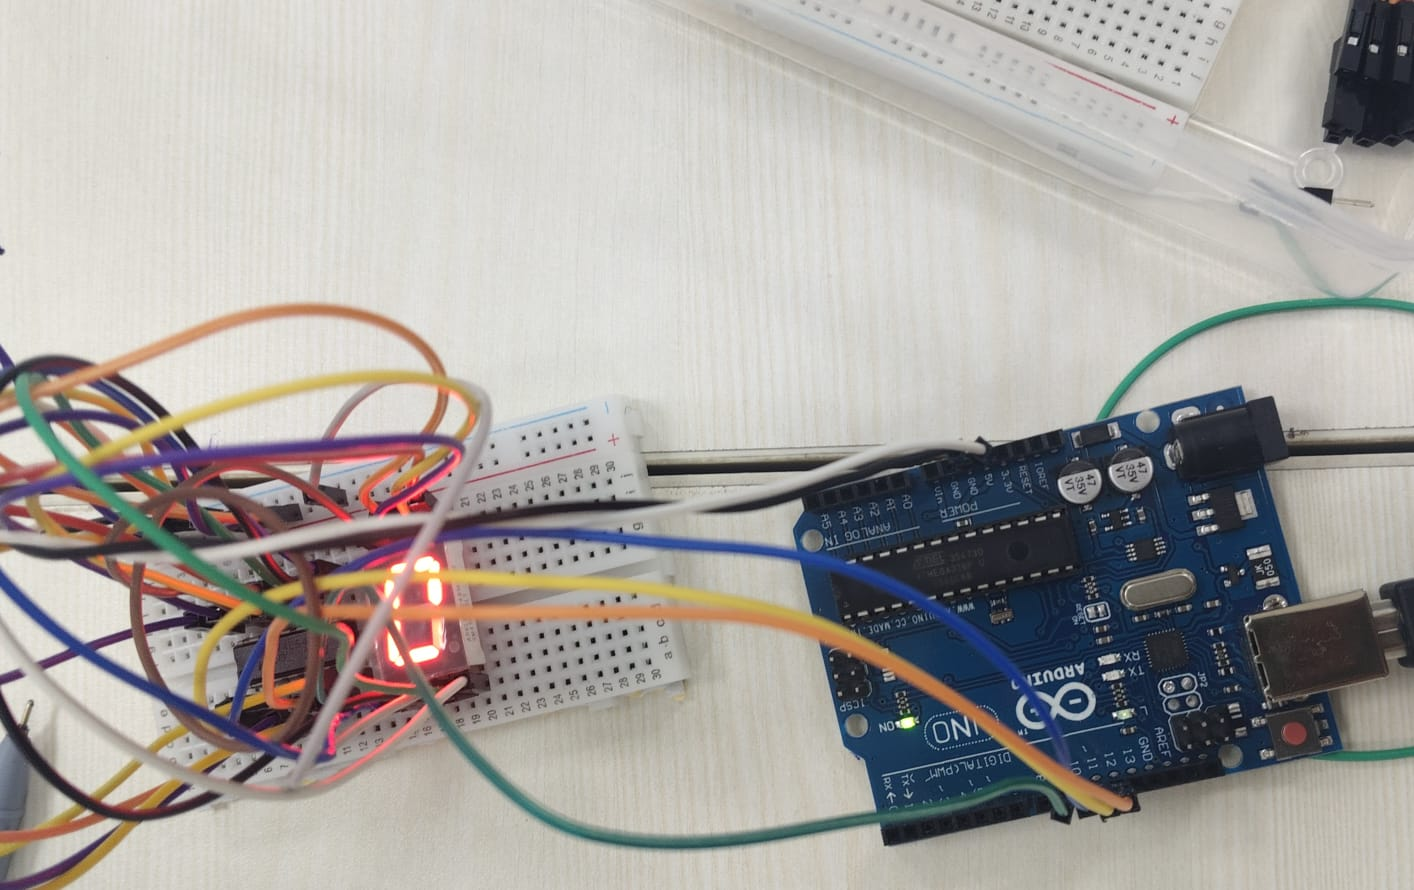
\includegraphics[width=0.5\textwidth]{output_0.jpeg}
\newline\newline
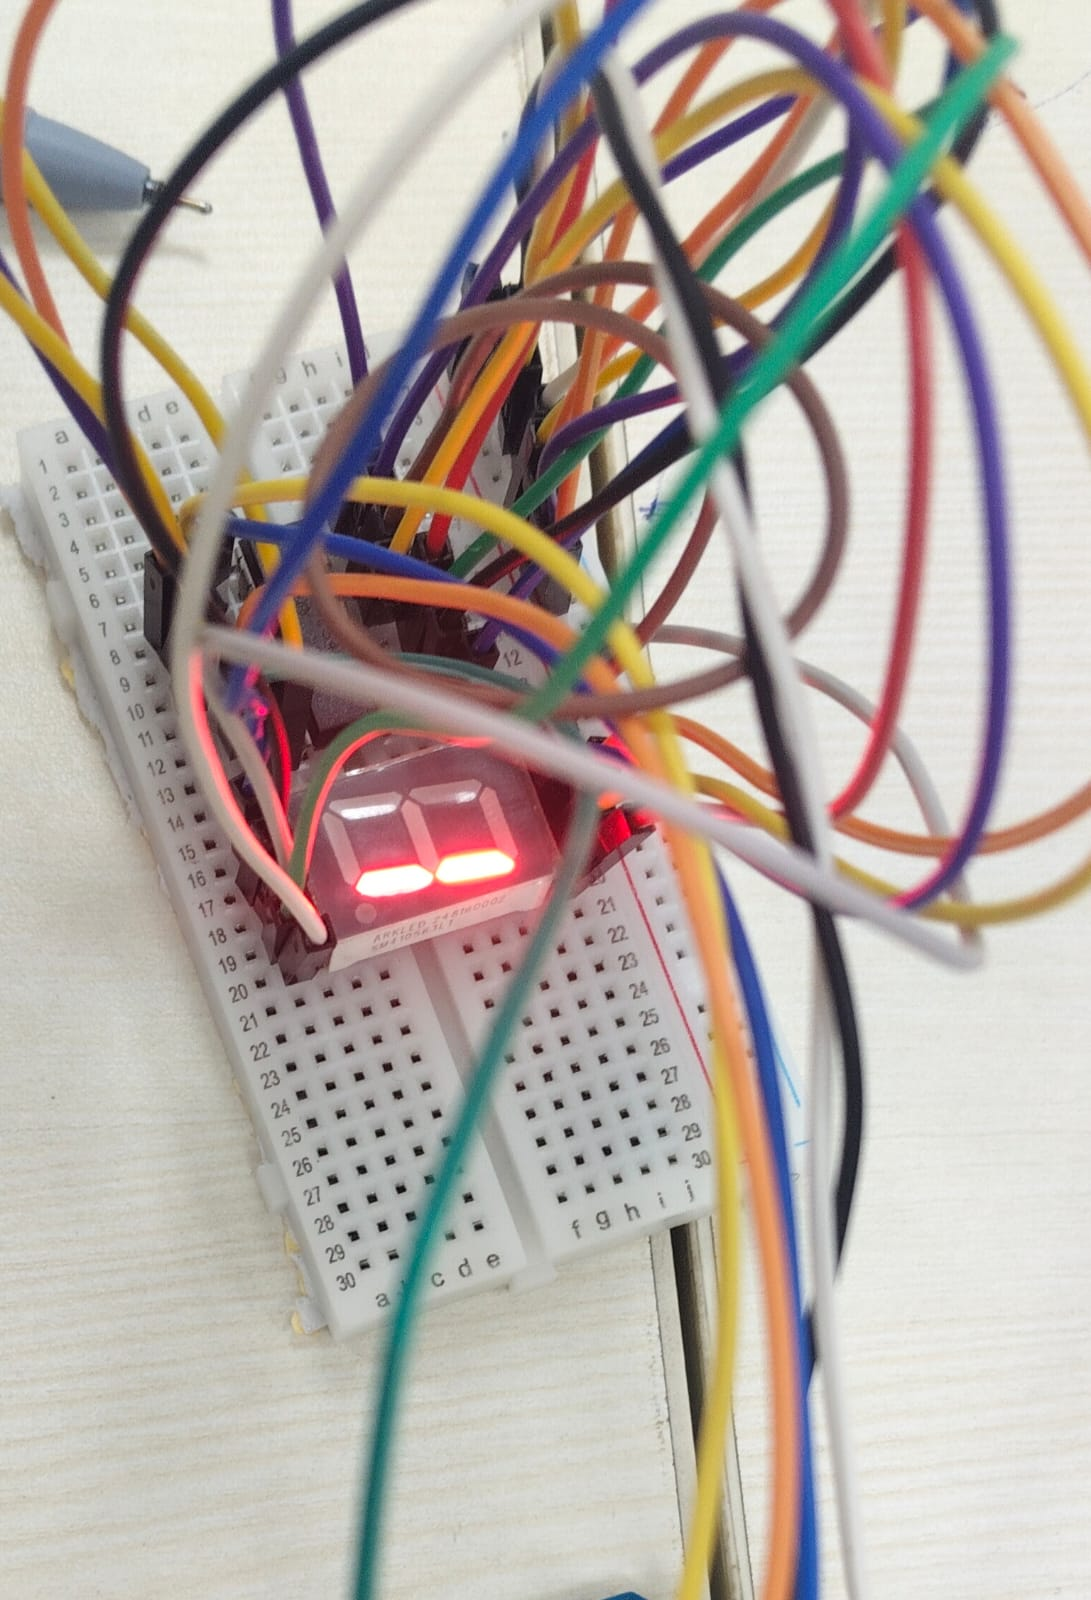
\includegraphics[width=0.5\textwidth]{Output_1.jpeg}
The simplified expression was successfully implemented using Arduino Uno, SN74LS47N, and a Common Anode Seven-Segment Display. The output values of \(Y\) were correctly displayed on the seven-segment display for all sixteen possible input combinations.
\end{document}
